% Options for packages loaded elsewhere
\PassOptionsToPackage{unicode}{hyperref}
\PassOptionsToPackage{hyphens}{url}
%
\documentclass[
]{article}
\usepackage{amsmath,amssymb}
\usepackage{lmodern}
\usepackage{ifxetex,ifluatex}
\ifnum 0\ifxetex 1\fi\ifluatex 1\fi=0 % if pdftex
  \usepackage[T1]{fontenc}
  \usepackage[utf8]{inputenc}
  \usepackage{textcomp} % provide euro and other symbols
\else % if luatex or xetex
  \usepackage{unicode-math}
  \defaultfontfeatures{Scale=MatchLowercase}
  \defaultfontfeatures[\rmfamily]{Ligatures=TeX,Scale=1}
\fi
% Use upquote if available, for straight quotes in verbatim environments
\IfFileExists{upquote.sty}{\usepackage{upquote}}{}
\IfFileExists{microtype.sty}{% use microtype if available
  \usepackage[]{microtype}
  \UseMicrotypeSet[protrusion]{basicmath} % disable protrusion for tt fonts
}{}
\makeatletter
\@ifundefined{KOMAClassName}{% if non-KOMA class
  \IfFileExists{parskip.sty}{%
    \usepackage{parskip}
  }{% else
    \setlength{\parindent}{0pt}
    \setlength{\parskip}{6pt plus 2pt minus 1pt}}
}{% if KOMA class
  \KOMAoptions{parskip=half}}
\makeatother
\usepackage{xcolor}
\IfFileExists{xurl.sty}{\usepackage{xurl}}{} % add URL line breaks if available
\IfFileExists{bookmark.sty}{\usepackage{bookmark}}{\usepackage{hyperref}}
\hypersetup{
  pdftitle={Proving the selection weight ratio minimum},
  pdfauthor={Jonathan Mellon},
  hidelinks,
  pdfcreator={LaTeX via pandoc}}
\urlstyle{same} % disable monospaced font for URLs
\usepackage[margin=1in]{geometry}
\usepackage{color}
\usepackage{fancyvrb}
\newcommand{\VerbBar}{|}
\newcommand{\VERB}{\Verb[commandchars=\\\{\}]}
\DefineVerbatimEnvironment{Highlighting}{Verbatim}{commandchars=\\\{\}}
% Add ',fontsize=\small' for more characters per line
\usepackage{framed}
\definecolor{shadecolor}{RGB}{248,248,248}
\newenvironment{Shaded}{\begin{snugshade}}{\end{snugshade}}
\newcommand{\AlertTok}[1]{\textcolor[rgb]{0.94,0.16,0.16}{#1}}
\newcommand{\AnnotationTok}[1]{\textcolor[rgb]{0.56,0.35,0.01}{\textbf{\textit{#1}}}}
\newcommand{\AttributeTok}[1]{\textcolor[rgb]{0.77,0.63,0.00}{#1}}
\newcommand{\BaseNTok}[1]{\textcolor[rgb]{0.00,0.00,0.81}{#1}}
\newcommand{\BuiltInTok}[1]{#1}
\newcommand{\CharTok}[1]{\textcolor[rgb]{0.31,0.60,0.02}{#1}}
\newcommand{\CommentTok}[1]{\textcolor[rgb]{0.56,0.35,0.01}{\textit{#1}}}
\newcommand{\CommentVarTok}[1]{\textcolor[rgb]{0.56,0.35,0.01}{\textbf{\textit{#1}}}}
\newcommand{\ConstantTok}[1]{\textcolor[rgb]{0.00,0.00,0.00}{#1}}
\newcommand{\ControlFlowTok}[1]{\textcolor[rgb]{0.13,0.29,0.53}{\textbf{#1}}}
\newcommand{\DataTypeTok}[1]{\textcolor[rgb]{0.13,0.29,0.53}{#1}}
\newcommand{\DecValTok}[1]{\textcolor[rgb]{0.00,0.00,0.81}{#1}}
\newcommand{\DocumentationTok}[1]{\textcolor[rgb]{0.56,0.35,0.01}{\textbf{\textit{#1}}}}
\newcommand{\ErrorTok}[1]{\textcolor[rgb]{0.64,0.00,0.00}{\textbf{#1}}}
\newcommand{\ExtensionTok}[1]{#1}
\newcommand{\FloatTok}[1]{\textcolor[rgb]{0.00,0.00,0.81}{#1}}
\newcommand{\FunctionTok}[1]{\textcolor[rgb]{0.00,0.00,0.00}{#1}}
\newcommand{\ImportTok}[1]{#1}
\newcommand{\InformationTok}[1]{\textcolor[rgb]{0.56,0.35,0.01}{\textbf{\textit{#1}}}}
\newcommand{\KeywordTok}[1]{\textcolor[rgb]{0.13,0.29,0.53}{\textbf{#1}}}
\newcommand{\NormalTok}[1]{#1}
\newcommand{\OperatorTok}[1]{\textcolor[rgb]{0.81,0.36,0.00}{\textbf{#1}}}
\newcommand{\OtherTok}[1]{\textcolor[rgb]{0.56,0.35,0.01}{#1}}
\newcommand{\PreprocessorTok}[1]{\textcolor[rgb]{0.56,0.35,0.01}{\textit{#1}}}
\newcommand{\RegionMarkerTok}[1]{#1}
\newcommand{\SpecialCharTok}[1]{\textcolor[rgb]{0.00,0.00,0.00}{#1}}
\newcommand{\SpecialStringTok}[1]{\textcolor[rgb]{0.31,0.60,0.02}{#1}}
\newcommand{\StringTok}[1]{\textcolor[rgb]{0.31,0.60,0.02}{#1}}
\newcommand{\VariableTok}[1]{\textcolor[rgb]{0.00,0.00,0.00}{#1}}
\newcommand{\VerbatimStringTok}[1]{\textcolor[rgb]{0.31,0.60,0.02}{#1}}
\newcommand{\WarningTok}[1]{\textcolor[rgb]{0.56,0.35,0.01}{\textbf{\textit{#1}}}}
\usepackage{graphicx}
\makeatletter
\def\maxwidth{\ifdim\Gin@nat@width>\linewidth\linewidth\else\Gin@nat@width\fi}
\def\maxheight{\ifdim\Gin@nat@height>\textheight\textheight\else\Gin@nat@height\fi}
\makeatother
% Scale images if necessary, so that they will not overflow the page
% margins by default, and it is still possible to overwrite the defaults
% using explicit options in \includegraphics[width, height, ...]{}
\setkeys{Gin}{width=\maxwidth,height=\maxheight,keepaspectratio}
% Set default figure placement to htbp
\makeatletter
\def\fps@figure{htbp}
\makeatother
\setlength{\emergencystretch}{3em} % prevent overfull lines
\providecommand{\tightlist}{%
  \setlength{\itemsep}{0pt}\setlength{\parskip}{0pt}}
\setcounter{secnumdepth}{-\maxdimen} % remove section numbering
\ifluatex
  \usepackage{selnolig}  % disable illegal ligatures
\fi

\title{Proving the selection weight ratio minimum}
\author{Jonathan Mellon}
\date{13/12/2021}

\begin{document}
\maketitle

In my
\href{https://www.filedrawer.blog/post/minimum-post-strat-weight-is-response-rate/}{previous
post} I showed that the minimum inverse-probability weight in a simple
random sample should be equal to the response rate of the survey.
However, simple random samples are basically non-existent in the real
world, so I need to work out the equivalent constraint for complex
survey designs.

This post summarizes my progress so far towards doing that.

In that post I speculated that the constraint for \(i\)'s weight should
be:

\[
\frac{FinalWeight_i}{SelectionWeight_i} >= RR_{total}
\]

\hypertarget{does-it-work-in-practice}{%
\section{Does it work in practice?}\label{does-it-work-in-practice}}

After an hour of failing to work out an analytic proof, I thought it
would be worth doing a simulation to see whether this claim is at least
empirically true.

So let's do a simple two-stage sample where households are randomly
selected, then a respondent is randomly selected from that household.
This means that people in larger households have a lower probability of
selection. If you live alone there's a 100\% chance of selection,
whereas if you live

Rich people respond at 100\% and poor people respond at 30\%.

\begin{Shaded}
\begin{Highlighting}[]
\FunctionTok{options}\NormalTok{(}\AttributeTok{scipen=}\DecValTok{9999}\NormalTok{)}


\NormalTok{simRR }\OtherTok{\textless{}{-}} \ControlFlowTok{function}\NormalTok{(pop.n, poor.rr, rich.rr, sample.n, }\AttributeTok{big.hh.rich =}\NormalTok{ F) \{}
\NormalTok{  hhs }\OtherTok{\textless{}{-}} \FunctionTok{sample}\NormalTok{(}\DecValTok{1}\SpecialCharTok{:}\NormalTok{pop.n, }\AttributeTok{replace =}\NormalTok{ T)}
\NormalTok{  hhs }\OtherTok{\textless{}{-}} \FunctionTok{as.numeric}\NormalTok{(}\FunctionTok{factor}\NormalTok{(hhs))}
\NormalTok{  hh.sizes }\OtherTok{\textless{}{-}} \FunctionTok{table}\NormalTok{(hhs)[}\FunctionTok{as.character}\NormalTok{(hhs)]}
  
  \ControlFlowTok{if}\NormalTok{(big.hh.rich) \{}
\NormalTok{    wealth }\OtherTok{\textless{}{-}} \FunctionTok{ifelse}\NormalTok{(}\FunctionTok{rbinom}\NormalTok{(}\AttributeTok{size =} \DecValTok{1}\NormalTok{ , }\AttributeTok{prob =}\NormalTok{ (}\DecValTok{1} \SpecialCharTok{{-}}\NormalTok{ (}\DecValTok{1} \SpecialCharTok{/}\NormalTok{ hh.sizes)), }\AttributeTok{n=}\NormalTok{pop.n), }\StringTok{"Rich"}\NormalTok{, }\StringTok{"Poor"}\NormalTok{)}
\NormalTok{  \} }\ControlFlowTok{else}\NormalTok{ \{}
\NormalTok{    wealth }\OtherTok{\textless{}{-}} \FunctionTok{ifelse}\NormalTok{(}\FunctionTok{rbinom}\NormalTok{(}\AttributeTok{size =} \DecValTok{1}\NormalTok{ , }\AttributeTok{prob =} \FloatTok{0.5}\NormalTok{, }\AttributeTok{n=}\NormalTok{pop.n), }\StringTok{"Rich"}\NormalTok{, }\StringTok{"Poor"}\NormalTok{)}
\NormalTok{  \}}
  
  
\NormalTok{  sampled.hh }\OtherTok{\textless{}{-}} \FunctionTok{sample}\NormalTok{(}\FunctionTok{unique}\NormalTok{(hhs), sample.n, }\AttributeTok{replace =}\NormalTok{ F)}
\NormalTok{  sampled.people }\OtherTok{\textless{}{-}} \FunctionTok{c}\NormalTok{()}
  \ControlFlowTok{for}\NormalTok{(ii }\ControlFlowTok{in}\NormalTok{ sampled.hh)\{}
\NormalTok{    sampled.people }\OtherTok{\textless{}{-}} \FunctionTok{c}\NormalTok{(sampled.people, }\FunctionTok{sample}\NormalTok{(}\FunctionTok{rep}\NormalTok{(}\FunctionTok{which}\NormalTok{(hhs}\SpecialCharTok{==}\NormalTok{ii), }\DecValTok{2}\NormalTok{), }\DecValTok{1}\NormalTok{))}
\NormalTok{  \}}
  
\NormalTok{  wealth.sampled }\OtherTok{\textless{}{-}}\NormalTok{ wealth[sampled.people]}
\NormalTok{  respondents }\OtherTok{\textless{}{-}}\NormalTok{ sampled.people[}
\NormalTok{    (wealth.sampled}\SpecialCharTok{==}\StringTok{"Poor"}\NormalTok{) }\SpecialCharTok{\&}\NormalTok{ (}\FunctionTok{rbinom}\NormalTok{(}\AttributeTok{n=}\NormalTok{sample.n, }\AttributeTok{prob =}\NormalTok{ poor.rr, }\AttributeTok{size =} \DecValTok{1}\NormalTok{)}\SpecialCharTok{==}\DecValTok{1}\NormalTok{) }\SpecialCharTok{|} 
\NormalTok{      (wealth.sampled}\SpecialCharTok{==}\StringTok{"Rich"}\NormalTok{) }\SpecialCharTok{\&}\NormalTok{ (}\FunctionTok{rbinom}\NormalTok{(}\AttributeTok{n=}\NormalTok{sample.n, }\AttributeTok{prob =}\NormalTok{ rich.rr, }\AttributeTok{size =} \DecValTok{1}\NormalTok{)}\SpecialCharTok{==}\DecValTok{1}\NormalTok{)]}
  
  \FunctionTok{prop.table}\NormalTok{(}\FunctionTok{table}\NormalTok{(wealth[respondents]))}
\NormalTok{  respondent.hh.size }\OtherTok{\textless{}{-}} \FunctionTok{table}\NormalTok{(hhs)[}\FunctionTok{as.character}\NormalTok{(hhs[respondents])]}
\NormalTok{  probability.selection }\OtherTok{\textless{}{-}}\NormalTok{ (sample.n }\SpecialCharTok{/} \FunctionTok{length}\NormalTok{(}\FunctionTok{unique}\NormalTok{(hhs))) }\SpecialCharTok{*} 
\NormalTok{    (}\DecValTok{1}\SpecialCharTok{/}\NormalTok{ respondent.hh.size)}
  
\NormalTok{  poor.rr.obs }\OtherTok{\textless{}{-}} \FunctionTok{sum}\NormalTok{(wealth[respondents]}\SpecialCharTok{==}\StringTok{"Poor"}\NormalTok{) }\SpecialCharTok{/} \FunctionTok{sum}\NormalTok{(wealth.sampled}\SpecialCharTok{==}\StringTok{"Poor"}\NormalTok{)}
  
\NormalTok{  probability.response }\OtherTok{\textless{}{-}}\NormalTok{ probability.selection }\SpecialCharTok{*} 
    \FunctionTok{ifelse}\NormalTok{(wealth[respondents]}\SpecialCharTok{==}\StringTok{"Rich"}\NormalTok{, rich.rr, poor.rr.obs)}
  
\NormalTok{  weights }\OtherTok{\textless{}{-}}\NormalTok{ (}\DecValTok{1} \SpecialCharTok{/}\NormalTok{ probability.response)}
\NormalTok{  selection.weights }\OtherTok{\textless{}{-}}\NormalTok{ (}\DecValTok{1} \SpecialCharTok{/}\NormalTok{ probability.selection)}
  
\NormalTok{  scaled.weights }\OtherTok{\textless{}{-}}\NormalTok{ weights }\SpecialCharTok{/} \FunctionTok{mean}\NormalTok{(weights)}
\NormalTok{  scaled.selection.weights }\OtherTok{\textless{}{-}}\NormalTok{ selection.weights }\SpecialCharTok{/} \FunctionTok{mean}\NormalTok{(selection.weights)}
\NormalTok{  ratios }\OtherTok{\textless{}{-}}\NormalTok{ scaled.weights }\SpecialCharTok{/}\NormalTok{ scaled.selection.weights}
\NormalTok{  ratios2 }\OtherTok{\textless{}{-}}\NormalTok{ weights }\SpecialCharTok{/}\NormalTok{ (selection.weights) }
\NormalTok{  ratios3 }\OtherTok{\textless{}{-}}\NormalTok{ ratios }\SpecialCharTok{/} \FunctionTok{mean}\NormalTok{(ratios)}
\NormalTok{  actual.rr }\OtherTok{\textless{}{-}} \FunctionTok{length}\NormalTok{(respondents) }\SpecialCharTok{/}\NormalTok{ sample.n}
  
\NormalTok{  out }\OtherTok{\textless{}{-}} \FunctionTok{list}\NormalTok{(}\AttributeTok{scaled.weights =}\NormalTok{ scaled.weights, }
              \AttributeTok{scaled.selection.weights =}\NormalTok{ scaled.selection.weights, }
              \AttributeTok{ratios =}\NormalTok{ ratios, }\AttributeTok{ratios2 =}\NormalTok{ ratios2,}
              \AttributeTok{ratios3 =}\NormalTok{ ratios3,}
              \AttributeTok{actual.rr =}\NormalTok{ actual.rr)}
  \FunctionTok{return}\NormalTok{(out)}
\NormalTok{\}}

\NormalTok{output }\OtherTok{\textless{}{-}} \FunctionTok{simRR}\NormalTok{(}\AttributeTok{pop.n =} \DecValTok{10000}\NormalTok{, }\AttributeTok{poor.rr =} \FloatTok{0.3}\NormalTok{, }\AttributeTok{rich.rr =} \DecValTok{1}\NormalTok{, }\AttributeTok{sample.n =} \DecValTok{1000}\NormalTok{, }\AttributeTok{big.hh.rich =}\NormalTok{ F)}
\end{Highlighting}
\end{Shaded}

So after simulating that I look at the response rate for the simulation
0.631 and the minimum value of the ratios of the final true weight to
the selection weight 0.63. Not far off, but not identical to the
response rate. So, it looks like my initial claim is on the right track
but not exactly right.

Let's try this a few more times and see whether it's robust.

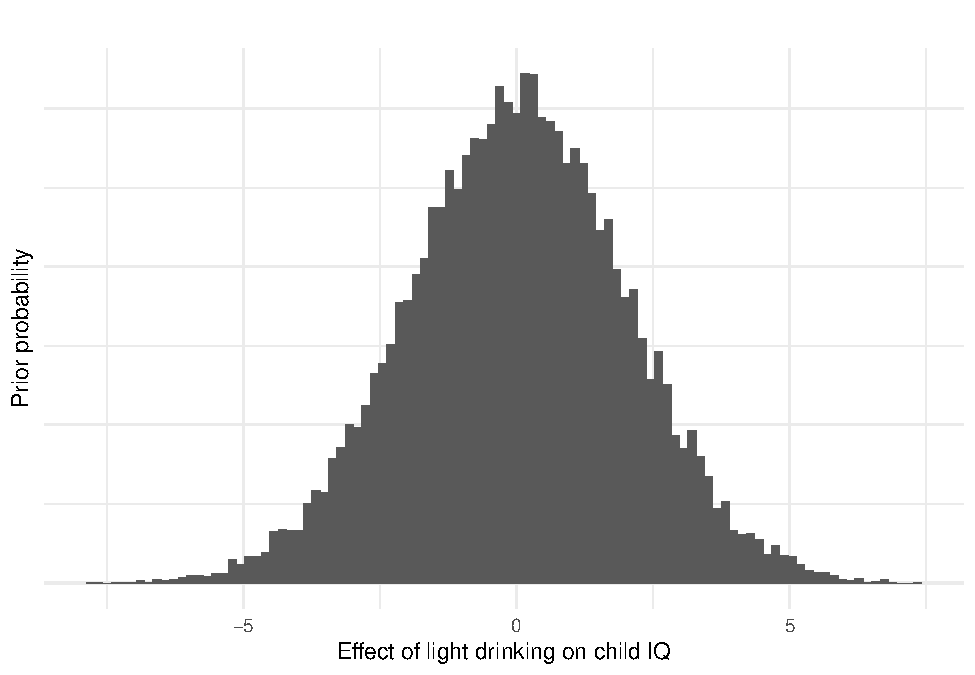
\includegraphics{selectionweightratio_files/figure-latex/unnamed-chunk-2-1.pdf}

After 100 simulations, it's clear there's a very strong relationship,
but this isn't an exact match.

OK, so what's going on with those ratios? The mean of the scaled
inverse-probability weights is always exactly 1 in the simulation.

Strangely, R doesn't think the mean of the scaled selection weights is
always exactly 1, although if you round to 10 decimal places it does, so
this is probably a floating point problem.

However, the ratios themselves are not always this close to zero. In
fact on average, they are 0.0103 away from zero. But do we actually
expect these ratios to be near one on average? If I simulate two random
vectors and rescale them to both have a mean of 1, the average ratio of
them isn't usually anywhere near 1.

\begin{Shaded}
\begin{Highlighting}[]
\FunctionTok{set.seed}\NormalTok{(}\DecValTok{1298}\NormalTok{)}
\NormalTok{A }\OtherTok{\textless{}{-}} \FunctionTok{abs}\NormalTok{(}\FunctionTok{rnorm}\NormalTok{(}\DecValTok{1000}\NormalTok{))}
\NormalTok{B }\OtherTok{\textless{}{-}} \FunctionTok{abs}\NormalTok{(}\FunctionTok{rnorm}\NormalTok{(}\DecValTok{1000}\NormalTok{))}
\NormalTok{A }\OtherTok{\textless{}{-}}\NormalTok{ A }\SpecialCharTok{/} \FunctionTok{mean}\NormalTok{(A)}
\NormalTok{B }\OtherTok{\textless{}{-}}\NormalTok{ B }\SpecialCharTok{/} \FunctionTok{mean}\NormalTok{(B)}
\FunctionTok{mean}\NormalTok{(A}\SpecialCharTok{/}\NormalTok{B)}
\end{Highlighting}
\end{Shaded}

\begin{verbatim}
## [1] 4.292947
\end{verbatim}

OK well what if I rescale the ratios so that they actually have a mean
of 1 rather than just being close to that?

\includegraphics{selectionweightratio_files/figure-latex/unnamed-chunk-7-1.pdf}

Apparently, that nails the minimum weight exactly. The mean absolute
difference between this adjusted ratio and the response rate for the
survey is just 0.000000000000000077715611723761. At that point I'm
willing to believe any remaining differences are just about floating
point precision.

\hypertarget{does-this-work-with-different-simulation-parameters}{%
\section{Does this work with different simulation
parameters?}\label{does-this-work-with-different-simulation-parameters}}

OK well first of all, let's make sure this actually holds up in a more
complex simulation. I'll set the poor response rate to 40\% and say that
people in bigger households are more likely to be rich (so that we have
a correlation between selection probability and group response rates).

Apparently this fix still works and the adjusted ratios exactly match
the response rate.

\begin{Shaded}
\begin{Highlighting}[]
\FunctionTok{ggplot}\NormalTok{(sims3, }\FunctionTok{aes}\NormalTok{(}\AttributeTok{x =}\NormalTok{ rr, }\AttributeTok{y =}\NormalTok{ ratioadj)) }\SpecialCharTok{+} \FunctionTok{geom\_point}\NormalTok{() }\SpecialCharTok{+} \FunctionTok{geom\_abline}\NormalTok{()}\SpecialCharTok{+} 
  \FunctionTok{xlab}\NormalTok{(}\StringTok{"Simulation response rate"}\NormalTok{) }\SpecialCharTok{+} 
  \FunctionTok{ylab}\NormalTok{(}\StringTok{"Final weight divided by selection weight (rescaling applied)"}\NormalTok{) }\SpecialCharTok{+} 
  \FunctionTok{theme\_minimal}\NormalTok{()}
\end{Highlighting}
\end{Shaded}

\includegraphics{selectionweightratio_files/figure-latex/unnamed-chunk-9-1.pdf}

\hypertarget{summarizing-the-claim}{%
\section{Summarizing the claim}\label{summarizing-the-claim}}

So to formalize, it looks like the constraint works as follows. For each
respondent, \(j\), define:

\[
r_j = \frac{FinalWeight_j}{SelectionWeight_j}
\]

The adjusted ratio is defined as follows, where \(\bar{r}\) is the mean
ratio across all respondents to the survey:

\[
r^{*}_j = \frac{r_j}{\bar{r}}
\] Based on my simulations, it appears that:

\[
r^{*}_{j}>= RR_{total}
\]

\hypertarget{but-why-does-this-work}{%
\section{But why does this work?}\label{but-why-does-this-work}}

🤷

\end{document}
